\documentclass[10pt, a4paper]{article}

%\usepackage{a4wide}
\usepackage[pdftex]{graphicx}
\usepackage{verbatim} 
\usepackage{ulem}
\usepackage{hyperref}
\usepackage[danish]{babel}
\usepackage{t1enc}
\usepackage{wrapfig} % wrapper til images (align in tekst)
\usepackage{amsmath,amssymb} % American Mathematical Society
\usepackage{listings}
\usepackage{fancyvrb}
\usepackage{clrscode} % algoritmer som brugt i bogen CLRS (2nd ed.)
\usepackage{mdwlist} % tighter lists when starred
%\usepackage{adjustbox} % allow shrinking of figures. % requires collectbox.sty

% Flow charts: 
\usepackage{tikz}
\usetikzlibrary{shapes,arrows}

% Italic theta and omega
\let\OldTheta\Theta
\renewcommand{\Theta}{\varTheta}
\let\OldOmega\Omega
\renewcommand{\Omega}{\varOmega}

% Til linieret kodeeksempler:
% \VerbatimInput[frame=leftline,numbers=left,numbersep=6pt]{<FILE>}
% Look at minted package for better code inclusions.

%declare where to look for graphics
\graphicspath{{gfx/}}

\newenvironment{sbrlist}
{\begin{description} \itemsep1pt \parskip0pt \parsep0pt}
{\end{description}}

\newcommand{\sbrbox}[1]
{\begin{center} \fbox{\begin{minipage}{0.92\linewidth}
    #1
\end{minipage}} \end{center}}

\begin{document}

%include everything
\title{\huge Distribuerede Systemer \\
       \small Afleveringsopgave - 5 - uge6 }
\author{Hold: DA4; Gruppe: 2\\ \\
        \href{mailto:skeen@cs.au.dk}{Emil Madsen - 20105376}\\
        \href{mailto:emray@cs.au.dk}{Rasmus - 20105109}\\
        \href{mailto:sverre@cs.au.dk}{Sverre - 20083549}
       }
\date{\today}

\maketitle

\hrule

\section*{Introduction}
    % each point and each class (how solved)
    Opgaven vi bliver stillet g�r ud p� at skrive et distributeret java chat
program, kaldet MultiChat. 
Programmet skal �ge vores evner til at forst� og arbejde med 'message passing
interfaces'.
For at l�se opgaven er en del kode udleveret.

Denne kode har vi, f�r vi begyndte at udf�re selve opgaven, valgt at
genneml�se, for at forst�.
Vi har i l�bet af denne process �ndret sm� ting, som f.eks. at tilf�je final og
lignende.
Vi har derefter, da vi ville igang med at kode vores l�sning, flyttet al den
udleverede kode ind i en pakke kaldet 'multicastqueue'.
For at dette skulle virke har vi v�ret n�dt til at tilf�je public til
klasserne, s�ledes at de kan tilg�s uden for den specifikke pakke.

Vi har valgt at kode vores version af MultiChat, vha. to prim�re tr�de, hvor
den ene h�ndterer input (at l�se brugerens input, samt at sende det), og den
hvor den anden tr�d s�rger for output (alts� at l�se indkomne beskeder og
skrive dem til sk�rmen). 
Dette giver os nem forst�elig kode, hvor ansvarene er p�nt opdelt.

De f�lgende krav var stillet til MultiChat-programmet;
\begin{enumerate*}
\item Hvis programmet startes uden argumenter, skal det starte en ny gruppe,
    med sig selv som eneste bruger.
\item Hvis programmet startes med et enkelt argument, skal dette argument
tolkes som navnet p� en v�rt, som er en del af en MultiChat gruppe, hvorefter
programmet skal blive en del af denne gruppe.
\item Hvis programmet modtager input strengen 'exit <ENTER>' skal det forlade
gruppen, og terminere.
\item N�r en instans af programmet lukkes ned, skal det lukkes fuldst�ndigt,
    det m� alts� ikke fungere som server for systemet. Dette g�lder selvom,
    denne specifikke maskine startede den aktuelle gruppe. Alts� m� systemet
    ikke benytte sig af en central server.
\item N�r en instans af programmet opretter forbindelse til en gruppe,
    forventes det, at al tidligere chat udskrives til terminalen.
\end{enumerate*}

I vores kode har vi opn�et disse m�l p� f�lgende m�der;
\begin{enumerate*}
\item I main metoden af programmet tjekkes antallet af argumenter til
programmet. 
Hvis dette er nul, kaldes 'MulticastQueue.createGroup()', med programmets
default-port\footnote{Vi har indstillet \proc{default-port} til at v�re 0, hvilket betyder styresystemet angiver en port. Dette tillader os at k�re flere instanser af MultiChat-programmet fra den samme pc.}, hvorefter programmet g�r til hovedl�kken (chat-delen).
\item Hvis vi derimod finder mindst 1 argument i main metoden, antager vi at
f�rste argument er et hostname, hvorefter vi parser strengen for at isolere
portnummer og v�rtsstreng.
N�r disse er fundet kalder vi 'MulticastQueue.joinGroup()' med de givne
parametre, hvorefter programmet (efter koden for krav-5) g�r til hovedl�kken.
\item I hovedl�kken oprettes som tidligere n�vnt to tr�de.
Krav 3 er fuldkommen indeholdt i input-tr�den, hvor vi simpelthen blot tjekker
den givne input tr�d imod strengen 'exit <ENTER>' og hvis et match findes
disconnecter og terminerer programmet.
\item Dette krav er opfyldt for os, da MulticastQueue sikrer en distributeret
messageQueue.
Alts� kan vi blot disconnecte og kanalen forbliver intakt.
\item Det er her den egentlige opgave ligger.
\subparagraph*{\footnotesize (�ndret i genafleveringen )}
Vi har for at opfylde kravet lavet en Multicast-QueueHistoryDecorator-klasse,
som giver ekstra funktionalitet og ellers bare f�rer metodekald videre til en
MulticastQueueFifoOnly instans.

Der bruges en speciel streng som payload i en MulticastMessagePayload, hvilken
er afsendt af MultiChat klassen, og denne h�ndteres af HistoryDecoratorens'
get() metode, men bliver ikke returneret.

Denne specielle besked bliver multicastet til alle p� netv�rket og indeholder
en retur addresse, som alle peers vil oprette en PointToPointQueue til for at
sende en MulticastMessagePayload med en arrayliste over alle tidligere
beskeder.
Afsenderen vil tage imod den f�rste s�danne besked og behandle de indeholdte beskeder.
\end{enumerate*}

Den generelle chat-klient er, som tidligere n�vnt, implementeret vha. to simple
tr�de, hvor input-tr�den blot l�ser brugerens input og sender det via message
systemet, og hvor output-tr�den blot l�ser fra message-systemet og skriver til
sk�rmen.
Vi mente den oplagte l�sning var to tr�de, da vi havde behov for at
udf�re to blokerende IO kald samtidigt.

S�ledes er alle de givne 5 punkter l�st i f�lge med opgavebeskrivelsen, og vi
har, som opgaven specificerer, udelukkende gjort brug af det udleverede kode,
til kontakten imellem klienterne.

\subsection*{Note}

Vi har udover al det tidligere n�vnte ogs� lavet et par sm� interface-�ndringer
i det udleverede kode.
Helt specifikt har vi �ndret 'PointToPointQueueReceiverEnd.listenOnPort(port)'
til at returnere en integer i stedet for void, da vi s�ledes har kunnet �ndre
internt i 'MulticastQueueFifoOnly' for at denne automatisk kan finde en port,
hvis den gives '0' som port-argument\footnote{I det indleverede kode er
default-porten 0, s�ledes at chat clienten blot starter p� en tilf�ldig fri
port}.
 

\subsection*{Klasse beskrivelse}

\begin{figure*}[htb]
\center
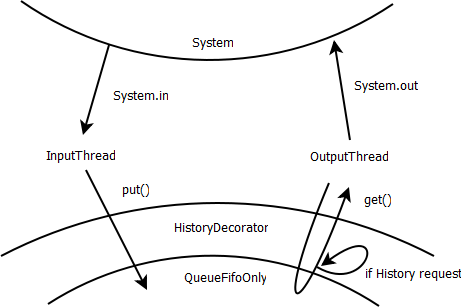
\includegraphics[width=0.74\textwidth]{uge3_threads}
\caption{Skitse af vores design med 2 tr�de og persistent history.}
\end{figure*}

Vores kode best�r af 4 nye klasser, som f�lger:

\begin{description}
\item[MultiChat]
Dette er 'main'-klassen.
Den opretter de relevante objecter og starter Input- og OutputThread.

Den indeholeer desuden delte resourser, som tilg�es static s�som Arraylisten
History, vores brugte portnumre og hostnavn.

Hvis man joiner en gruppe, er det ogs� MultiChat, der laver anmodning om
History fra peers, efter at man har sluttet sig til et netv�rk men f�r io-tr�dene startes.

Til sidst vil denne fores�ge at joine InputThread, s� k�rslen kan afsluttes, n�r
inputtr�den synes.

\item[InputThread]
Denne l�ser strenge fra konsollen via System.in og venter(/blokeres) indtil et linjeskift forekommer.
Den ignorerer tomme strenge og afsluttes, hvis brugeren skriver "exit <Enter>".

Alle ikke-tomme strenge, der l�ses fra konsollen, som ikke er et exit, bliver sat i MulticastQueue via put().


\item[OutputThread]
Output l�ser fra queue via get() og tjekker om en message er en instans af de 3
kendte message typer.
I det tilf�lde l�gges den i History-listen og en
passende besked skrives til konsollen.


\item[MulticastQueueHistoryDecorator]
Implementerer MessageQueue-interfacet og opfylder det ved at indeholde et
MulticastQueueFifoOnly object og passere alle metodekald til det. 

Den eksisterer kun for at lave speciel behandling af anmoodninger for gammel
history, hvilket alt sammen blot findes i dens get()-metode.

Anmodninger om history bliver ikke returneret, den pr�vet i stedet at lave
get() p� sin underl�ggende queue en gang til.
\end{description}


\section*{Questions}
    Derudover skulle vi besvare f�lgende sp�rgsm�l;

\subsubsection*{1. Do your implementation tolerate that two servers without
clients leave at the same time? Why / Why not? }
Da det eneste, der forbinder vores servere, er multicastqueuen, og da denne
nemt kan afbryde forbindelsen, ogs� concurrently, kan det sagtens lade sig g�re
at afbryde forbindelsen fra to servere samtidig.

\subsubsection*{2. Do your implementation implement the semantics of an atomic
section? If it does, how did you implement it?}
Vi har ikke implementeret atomic section, men vi kunne hurtigt g�re det, ved at
lave en speciel message type, der blot holder en liste af events, der s�
modtages som �n, og dermed ogs� udf�res som �n.



\section*{Usage Instructions}
    % how to test and run
    \subsection*{Kompilering}
Ant can bruges til at kompilere koden. 
Derefter kan man bruge java i terminalen fra build folderen.

Dvs. man kan starte vores regne server med 'java ServerTUIDistributed' og
clienten kan startes med 'java ClientTUI'

Eksempel for at kompilere og k�re i Windows:
\begin{verbatim}
...\kode>ant build
Buildfile: ...\kode\build.xml

prepare-build:

build-src:

build-test:
    [javac] ...

build:

BUILD SUCCESSFUL
Total time: 0 seconds

...\kode>cd build

...\kode\build>java ServerTUIDistributed
Exit: Gracefully logs out
Crash: Makes the server crash.

Enter address of another server (ENTER for standalone):
\end{verbatim}

Alternativt, kan man k�re de to bash scripts 'server.sh' og 'client.sh' for at
k�re de tilsvarende TUI's.

N�r en server startes, er der en foresp�rgsel om en server-adresse.
Hvis man undlader at skrive en adresse og blot trykker ENTER, vil serveren lave
en gruppe self.

For at forbinde til en eksisterende gruppe af servere skal man indtaste
\verb+<address>:<port>+.

Da porte oprettes dynamisk, skal man v�re opm�rksom p� at forbinde til den
server port, som er blevet bundet i den kendte peer.
 
I ClientTUI bliver man ligeledes spurgt om en server adresse.
Her skal man igen bruge \verb+<address>:<port>+.
% Todo : cleanup the following (duplicated?)
Bem�rk at dette er en anden port end 'server til server' porten.


\subsection*{Server ops�tning}
Den f�rste server der startes (den der skal lave server gruppen), skal ikke
gives noget argument, ved beskeden;
\begin{verbatim}
Enter address of another server (ENTER for standalone):
\end{verbatim}
Her skal vi alts� simpelt nok bare klikke '<ENTER>'.

For en server der skal joine en server gruppe, skal vi p� givne tidspunkt skrive
server group addressen p� den server vi �nsker at joine her; Denne findes nemt
ved at l�se outputtet fra en allerede k�rende server, og ser noglelunde s�ledes
ud;
\begin{verbatim}
...
Created/Joined server group at: llama04/10.11.82.4:53261
...
\end{verbatim}
Det er netop denne addresse der skal bruges, til at blive en del af server
gruppen. Dette skal indtastes med b�de addresse og navn, p� det s�dvanlige
'<address>:<port>' format. Man skal huske at kigge efter beskeden; 'Server
running', der indikere at serveren nu faktisk k�re.

\subsection*{Klient ops�tning}
For at kontakte til en server med en client skal man s�ledes ogs� kende noget
information fra serveren, nemlig p� hvilken port, den specifikke server,
servicere clienter, denne information er ligeledes nem at l�se, og ser
noglelunde s�ledes ud;
\begin{verbatim}
...
Listening for clients at: llama04/10.11.82.4:46814
...
\end{verbatim}
I clienten skal denne addresse, skrives p� samme format, som tidligere, n�r
beskeden;
\begin{verbatim}
Enter address of a server:
\end{verbatim}
Vises p� sk�rmen, herefter vil clienten udskrive information om, hvorvidt det
lykkedes at kontakte til serveren eller ej.
Noter venligst, at client porten, er anderledes en servergroup porten.



\section*{Conclusion}
    % write wrong or right
    Efter at have k�rt koden, er det muligt at l�seren har lagt m�rke til nogle sm�
defekter ved programmet. 
Dem der er kendt af udviklerne er:
\begin{itemize}
\item I tilf�lde af at flere peers opretter og afbryder forbindelsen til en
MultiChat-gruppe, forekommer der gentagelser af 'join'-beskeder i historien.
\item Der er problemer, hvis man pr�ver at forbinde til en MultiChat-peer p� \verb+localhost+ eller \verb+127.0.0.1+. Brug i stedet IP-adressen som konsollen angiver ved beskeder.
\end{itemize}

Vi konkluderer at vi har l�st opgaven med vores kode i tilfredsstillende grad,
da vi kan udf�re pr�cis den chat-sekvens som er fremvist i bunden af opgavebeskrivelsen.

\subsubsection*{Late additional note}
Vi har tilf�jet forkortelsen '\verb+ant mc+' for '\verb+ant multichat+'.

Vi har haft en succesfuld testsession over vpn p� tv�rs af OS's (llamaXX og egen windows pc).
Vi opdagede dog en masse forsinkelse s� l�nge flere peers var forbundet over vpn-forbindelsen.

Derudover har vi arbejdet med et \proc{gui} og \proc{cli}, hvor der dog stadig er lidt problemer.
Man kan tjekke de forskellige Ant targets vha. '\verb+ant help+.


 
% that's all folks
\end{document}
